\documentclass[11pt,a4paper]{article}
\usepackage[margin=2.7cm]{geometry}
\usepackage{amsmath,amssymb,amsthm,booktabs,tikz,microtype,float}
\usepackage[colorlinks,linkcolor=black,citecolor=black,urlcolor=blue!50!black]{hyperref}

\definecolor{curveC}{HTML}{111111}\definecolor{squareC}{HTML}{D1342F}
\definecolor{discC}{HTML}{2A7DE1}\definecolor{outerC}{HTML}{2A7DE1}
\definecolor{lostC}{HTML}{B9770E}\definecolor{dotC}{HTML}{111111}\definecolor{looseC}{HTML}{B9770E}

\newtheorem{theorem}{Theorem}
\newtheorem{proposition}[theorem]{Proposition}
\newtheorem{lemma}[theorem]{Lemma}
\newtheorem{corollary}[theorem]{Corollary}
\theoremstyle{remark}\newtheorem{remark}[theorem]{Remark}

\title{Inscribed squares can be small:\\ a counterexample to the big peg conjecture}
\author{Olli Paloviita}
\date{November 2026}

\begin{document}
\maketitle

\begin{abstract}
A square is inscribed in a closed curve if its four corners lie on the curve.
We give a family of $13$-gons that contain a disc of radius $2m$ but whose only
inscribed square has side less than $37$, for every $m\ge171$. This disproves the
big peg conjecture of Schwartz, which asked for an inscribed square of size
bounded below in terms of the inradius. Matschke's annulus theorem says that a
closed curve winding once around an annulus of inner radius $1$ and outer radius
$1+\sqrt2$ has an inscribed square of side at least $\sqrt2$; we show that the
outer radius cannot be increased beyond $2.4144$.
Both results are finite computations in exact rational arithmetic, and the
programs are short and public.
\end{abstract}

\noindent\textbf{Status.} The author is a software developer, not a mathematician.
The constructions, the computations and this text were produced by guiding coding
agents. The results were checked by programs written for the purpose and,
independently, by the exact programs of B.~J.~Schulz~\cite{schulz}, which agree
on every polygon tested (Section~5). No mathematician has reviewed them, and they
may contain mistakes. They are made public because they appear to close two
directions that cannot succeed. Every claim can be re-run from
\url{https://github.com/ollipal/small-inscribed-squares}; corrections are welcome there.

\section{Introduction}

Toeplitz asked in 1911 whether every Jordan curve in the plane has an inscribed
square. The answer is yes for smooth curves and for polygons, and open in
general. A natural plan is to approximate a curve by polygons and pass to the
limit; it fails only because the squares of the approximating polygons might
shrink to a point. Matschke's survey~\cite{matschke-survey} makes this explicit:
it would suffice that a piecewise linear curve containing a disc of radius $r$
inscribes a square of side at least $\varepsilon r$. Schwartz~\cite{schwartz}
stated it as a conjecture. Call a polygon \emph{wide} if the bounded component
of its complement contains a disc of radius~$1$.

\begin{quote}
\textbf{Conjecture 3.5 of \cite{schwartz} (Big peg conjecture).} There is some
$\varepsilon_0>0$ with the following property. Every wide polygon has an
inscribed square of sidelength at least~$\varepsilon_0$.
\end{quote}

\begin{theorem}\label{thm:rooms}
Let $P(m)$ be the $13$-gon with corners $m\,(x_i,y_i)+(dx_i,dy_i)$ given in
Table~\ref{tab:rooms}. For every real $m\ge171$, and also for
$m\in\{20,40,80,100\}$:
\begin{enumerate}
\item $P(m)$ is a simple polygon;
\item $P(m)$ contains the disc of radius $2m$ centred at $(3m,-4m)$;
\item $P(m)$ has exactly one inscribed square, and its side is less than $37$.
\end{enumerate}
\end{theorem}

\begin{corollary}
The big peg conjecture is false: for $m\ge171$, the polygon $P(m)$ scaled by
$1/(2m)$ is wide and its only inscribed square has side less than $18.5/m$.
\end{corollary}

The inscribed square problem itself is untouched, since every $P(m)$ has a square.
What fails is the hope of proving it by a size bound in terms of the inradius alone.

The second result concerns a setting where a size bound does hold. For $\rho>1$
let $A_\rho=\{x\in\mathbb R^2: 1\le\|x\|\le\rho\}$.
Matschke~\cite[Theorem~1.3]{matschke} proved that every closed curve in
$A_{1+\sqrt2}$ representing a generator of $\pi_1$ inscribes a square of side at
least $\sqrt2$, and remarked~\cite[Remark~2.6]{matschke} that for any
$\rho>1+\sqrt2$ it is open whether this holds for $A_\rho$.

\begin{theorem}\label{thm:ring}
For every $\rho\ge 2.4144$ there is a simple polygon in $A_\rho$, winding once
around the origin, all of whose inscribed squares have side less than $\sqrt2$.
\end{theorem}

Since $1+\sqrt2=2.41421\ldots$, the constant in Matschke's theorem is optimal to
within $2\cdot10^{-4}$, and the examples suggest that it is exactly optimal
(Section~4).

\paragraph{Earlier work.} The stronger guess that the bound is $\sqrt2$ times
the inradius, as for a circle, was posed as a challenge by D.~Bernier and
refuted by G.~Pochuev~\cite{pochuev} in August 2026 with a $10$-gon of ratio
$1.4104$; see Appendix~A and also~\cite{schulz}.
Schulz's research log~\cite{schulz} improves that ratio to $1.4084$, proves a
bound of this kind for several families of polygons, and names the existence of
some universal positive constant as the remaining question; Theorem~\ref{thm:rooms}
answers it in the negative. We are not aware of an earlier counterexample to the
conjecture as Schwartz states it, nor of an answer to Matschke's remark, but this
is an active area and we may have missed one.

\section{Method}

\begin{lemma}\label{lem:linear}
Write a square as $p,\;p+v,\;p+v+Rv,\;p+Rv$ with $R$ the quarter turn. Given four
lines $\ell_0,\dots,\ell_3$, the condition that the $j$-th corner lies on $\ell_j$
for each $j$ is a system of four linear equations in $(p,v)\in\mathbb R^4$.
\end{lemma}

Each corner is linear in $(p,v)$ and each line is one linear equation, so the
lemma is immediate. For a polygon with $n$ sides we solve the system for every
ordered choice of four sides, $n^4$ in all. A unique solution with $v\neq0$ is an
inscribed square exactly when each corner lies on its closed side. A singular but
consistent system is harmless if it forces $v=0$; otherwise it would signal a
sliding family of squares, which does not occur for the polygons below. With
rational corners every step is exact, so the list of inscribed squares is
complete and certain.

For a family $m\,(x_i,y_i)+(dx_i,dy_i)$ the same computation is done with $m$ as
a symbol. Every decision becomes the sign of a polynomial in $m$, which is
constant beyond its largest real root. Sturm sequences locate that root for each
of the $74162$ polynomials involved; the largest is below $171$. A disc centred at $c$ lies inside a
polygon if $c$ is inside and the exact distance from $c$ to every side is at
least the radius.

\section{Three rooms}

\begin{table}[H]\centering\small
\begin{tabular}{rrrrr@{\qquad\qquad}rrrrr}\toprule
$i$&$x$&$y$&$dx$&$dy$&$i$&$x$&$y$&$dx$&$dy$\\\midrule
1&$-8$&$0$&$0$&$3$&8&$6$&$-8$&$8$&$2$\\
2&$0$&$0$&$-3$&$-3$&9&$6$&$0$&$5$&$1$\\
3&$-6$&$0$&$3$&$-1$&10&$0$&$0$&$9$&$0$\\
4&$-6$&$-6$&$-2$&$1$&11&$0$&$0$&$0$&$9$\\
5&$0$&$-6$&$4$&$-2$&12&$0$&$6$&$4$&$1$\\
6&$0$&$0$&$3$&$-16$&13&$-7$&$6$&$-8$&$1$\\
7&$0$&$-7$&$7$&$-1$\\\bottomrule
\end{tabular}
\caption{The polygon $P(m)$: corner $i$ is $m\,(x_i,y_i)+(dx_i,dy_i)$.}\label{tab:rooms}
\end{table}

$P(m)$ consists of three \emph{rooms} of size about $6m$, in three quadrants,
meeting at a \emph{hub} of four corners that do not depend on~$m$
(Figure~\ref{fig:rooms}). Two thin slits separate neighbouring rooms.

\begin{figure}[H]\centering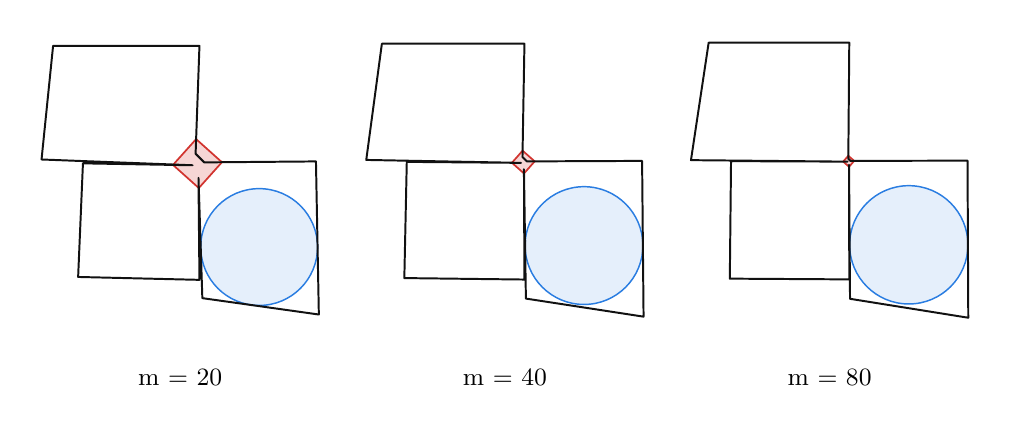
\begin{tikzpicture}[x=0.01250cm,y=0.01250cm,line join=round]
\begin{scope}\clip (15.0,-10.0) rectangle (325.0,-320.0);\path[line width=0.0187cm, draw=discC, fill=discC, fill opacity=0.12] (250.24,-232.94) circle (59.36);\end{scope}
\begin{scope}\clip (15.0,-10.0) rectangle (325.0,-320.0);\path[line width=0.0219cm, draw=squareC, fill=squareC, fill opacity=0.2] (162.69,-149.48) -- (188.93,-172.97) -- (212.42,-146.74) -- (186.19,-123.25) -- cycle;\end{scope}
\begin{scope}\clip (15.0,-10.0) rectangle (325.0,-320.0);\path[line width=0.0250cm, draw=curveC] (29.09,-143.96) -- (182.72,-149.83) -- (71.17,-147.88) -- (66.28,-263.34) -- (189.57,-266.28) -- (188.59,-162.55) -- (192.51,-284.87) -- (310.91,-301.51) -- (307.97,-145.92) -- (194.46,-146.90) -- (185.66,-138.09) -- (189.57,-28.49) -- (40.83,-28.49) -- cycle;\end{scope}
\node[font=\small] at (170.0,-365.0) {m $=$ 20};
\begin{scope}\clip (345.0,-10.0) rectangle (655.0,-320.0);\path[line width=0.0187cm, draw=discC, fill=discC, fill opacity=0.12] (580.38,-231.44) circle (59.85);\end{scope}
\begin{scope}\clip (345.0,-10.0) rectangle (655.0,-320.0);\path[line width=0.0219cm, draw=squareC, fill=squareC, fill opacity=0.2] (507.12,-147.31) -- (519.42,-158.16) -- (530.27,-145.86) -- (517.97,-135.01) -- cycle;\end{scope}
\begin{scope}\clip (345.0,-10.0) rectangle (655.0,-320.0);\path[line width=0.0250cm, draw=curveC] (359.09,-144.41) -- (516.37,-147.39) -- (400.27,-146.39) -- (397.79,-264.48) -- (519.85,-265.97) -- (519.35,-153.84) -- (521.33,-285.32) -- (640.91,-303.68) -- (639.42,-145.40) -- (522.33,-145.90) -- (517.86,-141.43) -- (519.85,-26.32) -- (374.97,-26.32) -- cycle;\end{scope}
\node[font=\small] at (500.0,-365.0) {m $=$ 40};
\begin{scope}\clip (675.0,-10.0) rectangle (985.0,-320.0);\path[line width=0.0187cm, draw=discC, fill=discC, fill opacity=0.12] (910.45,-230.69) circle (60.11);\end{scope}
\begin{scope}\clip (675.0,-10.0) rectangle (985.0,-320.0);\path[line width=0.0219cm, draw=squareC, fill=squareC, fill opacity=0.2] (843.79,-146.12) -- (849.75,-151.34) -- (854.97,-145.38) -- (849.01,-140.16) -- cycle;\end{scope}
\begin{scope}\clip (675.0,-10.0) rectangle (985.0,-320.0);\path[line width=0.0250cm, draw=curveC] (689.09,-144.64) -- (848.24,-146.14) -- (729.81,-145.64) -- (728.57,-265.06) -- (849.99,-265.81) -- (849.74,-149.39) -- (850.74,-285.55) -- (970.91,-304.78) -- (970.16,-145.14) -- (851.24,-145.39) -- (848.99,-143.14) -- (849.99,-25.22) -- (707.08,-25.22) -- cycle;\end{scope}
\node[font=\small] at (830.0,-365.0) {m $=$ 80};
\end{tikzpicture}

\caption{$P(m)$ drawn at equal width, with the largest disc in the lower-right room and the
unique inscribed square. In true units the square stays about $30$ across while
the rooms grow.}\label{fig:rooms}
\end{figure}

\begin{proof}[Proof of Theorem~\ref{thm:rooms}]
By the computation of Section~2: for the four listed values of $m$ with rational
arithmetic (\texttt{verify.py}), and for all $m\ge171$ with $m$ symbolic
(\texttt{verify\_all\_m.py}). Of the $13^4$ choices of sides exactly one yields a
square; its side tends to $30.4795\ldots$ as $m\to\infty$.
\end{proof}

\begin{remark}[Why it works]
Close one room by a straight wall across its doorway. The resulting pentagon has
$1$, $3$ and $1$ inscribed squares for the three rooms respectively, all of the
size of the room, and each has a corner on the doorway wall
(Figure~\ref{fig:doorways}). In $P(m)$ that wall is absent, so none survives. A
single room cannot work: as such a square is moved with three corners on the
walls, its fourth corner leaves through the doorway, and if the exterior lies
beyond it must cross the boundary, creating a square. Further rooms let it pass
from interior to interior. That no large square has corners in several rooms we
know only from the computation.
\end{remark}

\begin{figure}[H]\centering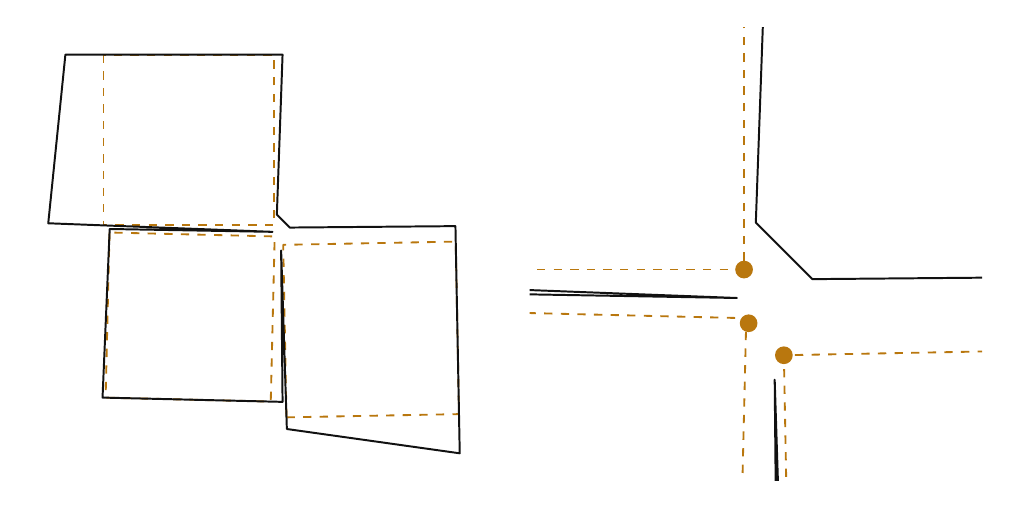
\begin{tikzpicture}[x=0.01250cm,y=0.01250cm,line join=round]
\begin{scope}\clip (20.0,-10.0) rectangle (480.0,-470.0);\path[line width=0.0234cm, draw=lostC, dashed] (97.03,-37.44) -- (97.03,-210.93) -- (270.52,-210.93) -- (270.52,-37.44) -- cycle;\end{scope}
\begin{scope}\clip (530.0,-10.0) rectangle (990.0,-470.0);\path[line width=0.0234cm, draw=lostC, dashed] (-15.27,507.50) -- (-15.27,-255.83) -- (748.06,-255.83) -- (748.06,507.50) -- cycle;\end{scope}
\begin{scope}\clip (530.0,-10.0) rectangle (990.0,-470.0);\path[fill=looseC, fill opacity=1] (748.06,-255.83) circle (9.00);\end{scope}
\begin{scope}\clip (20.0,-10.0) rectangle (480.0,-470.0);\path[line width=0.0234cm, draw=lostC, dashed] (103.19,-218.17) -- (99.20,-386.00) -- (267.03,-390.00) -- (271.03,-222.16) -- cycle;\end{scope}
\begin{scope}\clip (530.0,-10.0) rectangle (990.0,-470.0);\path[line width=0.0234cm, draw=lostC, dashed] (11.83,-287.68) -- (-5.75,-1026.16) -- (732.73,-1043.74) -- (750.31,-305.26) -- cycle;\end{scope}
\begin{scope}\clip (530.0,-10.0) rectangle (990.0,-470.0);\path[fill=looseC, fill opacity=1] (752.67,-310.37) circle (9.00);\end{scope}
\begin{scope}\clip (20.0,-10.0) rectangle (480.0,-470.0);\path[line width=0.0234cm, draw=lostC, dashed] (283.02,-406.03) -- (458.34,-402.73) -- (455.03,-227.41) -- (279.71,-230.71) -- cycle;\end{scope}
\begin{scope}\clip (530.0,-10.0) rectangle (990.0,-470.0);\path[line width=0.0234cm, draw=lostC, dashed] (803.06,-1114.30) -- (1574.47,-1099.75) -- (1559.92,-328.33) -- (788.50,-342.89) -- cycle;\end{scope}
\begin{scope}\clip (530.0,-10.0) rectangle (990.0,-470.0);\path[fill=looseC, fill opacity=1] (788.50,-342.89) circle (9.00);\end{scope}
\begin{scope}\clip (20.0,-10.0) rectangle (480.0,-470.0);\path[line width=0.0250cm, draw=curveC] (40.91,-208.78) -- (268.88,-217.49) -- (103.35,-214.59) -- (96.09,-385.93) -- (279.04,-390.28) -- (277.59,-236.37) -- (283.40,-417.87) -- (459.09,-442.56) -- (454.73,-211.69) -- (286.30,-213.14) -- (273.23,-200.07) -- (279.04,-37.44) -- (58.33,-37.44) -- cycle;\end{scope}
\begin{scope}\clip (530.0,-10.0) rectangle (990.0,-470.0);\path[line width=0.0250cm, draw=curveC] (-262.22,-246.39) -- (740.83,-284.72) -- (12.50,-271.94) -- (-19.44,-1025.83) -- (785.56,-1045.00) -- (779.17,-367.78) -- (804.72,-1166.39) -- (1577.78,-1275.00) -- (1558.61,-259.17) -- (817.50,-265.56) -- (760.00,-208.06) -- (785.56,507.50) -- (-185.56,507.50) -- cycle;\end{scope}
\end{tikzpicture}

\caption{Left: the squares each room of $P(20)$ would have with its doorway
closed. Right: the hub; the marked corners would need a wall in the doorway.}\label{fig:doorways}
\end{figure}


\section{The annulus theorem is nearly sharp}

A simple polygon $Q$ with a point $c$ in its interior lies in the annulus about
$c$ with inner radius $r$, the distance from $c$ to $Q$, and outer radius $R$, the
largest distance from $c$ to a corner; it winds once around~$c$. If every
inscribed square of $Q$ has side less than $\sqrt2\,r$, then $Q$ scaled by $1/r$
shows that the conclusion of Matschke's theorem fails in $A_\rho$ for every
$\rho\ge R/r$.

\begin{table}[H]\centering\small
\begin{tabular}{rlrrrr}\toprule
corners&centre $c$&$r$&largest side&$\sqrt2\,r$&$R/r$\\\midrule
5&$(16/3,\,16/3)$&$1.8856$&$2.5686$&$2.6667$&$3.1623$\\
8&$(49/5,\,129/10)$&$5.1800$&$7.2801$&$7.3256$&$2.6062$\\
12&$(641/10,\,3059/50)$&$21.9883$&$31.0644$&$31.0961$&$2.4340$\\
16&$(391/5,\,316/5)$&$25.6400$&$36.1146$&$36.2604$&$2.4238$\\
62&$(-93694,\,137563)$&$233986.0$&$329076.9$&$330906.2$&$2.41440$\\\bottomrule
\end{tabular}
\caption{Polygons violating the conclusion of Matschke's theorem in wider annuli.
The pentagon is that of Appendix~A; the others are listed in
the repository. All comparisons are exact; decimals are rounded.}\label{tab:ring}
\end{table}

\begin{figure}[H]\centering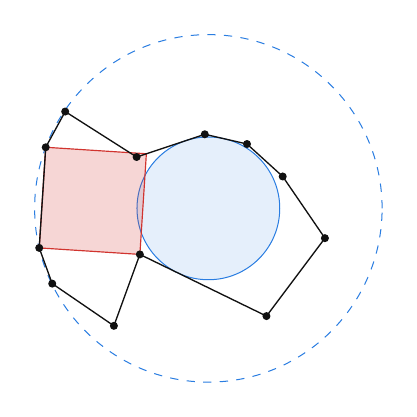
\begin{tikzpicture}[x=0.00850cm,y=0.00850cm,line join=round]
\begin{scope}\clip (230.0,-10.0) rectangle (770.0,-550.0);\path[line width=0.0128cm, draw=discC, fill=discC, fill opacity=0.12] (500.00,-280.00) circle (106.66);\end{scope}
\begin{scope}\clip (230.0,-10.0) rectangle (770.0,-550.0);\path[line width=0.0128cm, draw=outerC, dashed] (500.00,-280.00) circle (259.62);\end{scope}
\begin{scope}\clip (230.0,-10.0) rectangle (770.0,-550.0);\path[line width=0.0149cm, draw=squareC, fill=squareC, fill opacity=0.2] (407.35,-198.41) -- (256.97,-188.70) -- (247.26,-339.08) -- (397.64,-348.79) -- cycle;\end{scope}
\begin{scope}\clip (230.0,-10.0) rectangle (770.0,-550.0);\path[line width=0.0170cm, draw=curveC] (397.64,-348.79) -- (586.83,-440.96) -- (674.15,-324.53) -- (611.09,-232.36) -- (557.73,-183.85) -- (494.66,-169.30) -- (392.79,-203.26) -- (286.07,-135.34) -- (256.97,-188.70) -- (247.26,-339.08) -- (266.67,-392.45) -- (358.84,-455.51) -- cycle;\end{scope}
\begin{scope}\clip (230.0,-10.0) rectangle (770.0,-550.0);\path[fill=dotC, fill opacity=1] (397.64,-348.79) circle (6.00);\end{scope}
\begin{scope}\clip (230.0,-10.0) rectangle (770.0,-550.0);\path[fill=dotC, fill opacity=1] (586.83,-440.96) circle (6.00);\end{scope}
\begin{scope}\clip (230.0,-10.0) rectangle (770.0,-550.0);\path[fill=dotC, fill opacity=1] (674.15,-324.53) circle (6.00);\end{scope}
\begin{scope}\clip (230.0,-10.0) rectangle (770.0,-550.0);\path[fill=dotC, fill opacity=1] (611.09,-232.36) circle (6.00);\end{scope}
\begin{scope}\clip (230.0,-10.0) rectangle (770.0,-550.0);\path[fill=dotC, fill opacity=1] (557.73,-183.85) circle (6.00);\end{scope}
\begin{scope}\clip (230.0,-10.0) rectangle (770.0,-550.0);\path[fill=dotC, fill opacity=1] (494.66,-169.30) circle (6.00);\end{scope}
\begin{scope}\clip (230.0,-10.0) rectangle (770.0,-550.0);\path[fill=dotC, fill opacity=1] (392.79,-203.26) circle (6.00);\end{scope}
\begin{scope}\clip (230.0,-10.0) rectangle (770.0,-550.0);\path[fill=dotC, fill opacity=1] (286.07,-135.34) circle (6.00);\end{scope}
\begin{scope}\clip (230.0,-10.0) rectangle (770.0,-550.0);\path[fill=dotC, fill opacity=1] (256.97,-188.70) circle (6.00);\end{scope}
\begin{scope}\clip (230.0,-10.0) rectangle (770.0,-550.0);\path[fill=dotC, fill opacity=1] (247.26,-339.08) circle (6.00);\end{scope}
\begin{scope}\clip (230.0,-10.0) rectangle (770.0,-550.0);\path[fill=dotC, fill opacity=1] (266.67,-392.45) circle (6.00);\end{scope}
\begin{scope}\clip (230.0,-10.0) rectangle (770.0,-550.0);\path[fill=dotC, fill opacity=1] (358.84,-455.51) circle (6.00);\end{scope}
\end{tikzpicture}

\caption{The $12$-gon of Table~\ref{tab:ring}:
$(43,47)$, $(82,28)$, $(100,52)$, $(87,71)$, $(76,81)$, $(63,84)$, $(42,77)$,
$(20,91)$, $(14,80)$, $(12,49)$, $(16,38)$, $(35,25)$. Its only inscribed square
has side $\sqrt{965}$.}
\end{figure}

\begin{proof}[Proof of Theorem~\ref{thm:ring}]
The last row of Table~\ref{tab:ring}, verified by \texttt{verify.py --slow}:
the $62$-gon has eleven inscribed squares, the largest of side
$1.40640\,r<\sqrt2\,r$, and $R/r<2.41440$.
\end{proof}

The ratio fell steadily as corners were added (Table~\ref{tab:ring}), and the
search that produced the $62$-gon was still improving when it was stopped. We
expect that more complicated polygons come arbitrarily close to $1+\sqrt2$, which
would make Matschke's constant exactly optimal, but we have not proved this.
Simple examples already exist a little further out: the $8$-gon
$(-2,7)$, $(4,12)$, $(13,0)$, $(16,17)$, $(6,19)$, $(7,26)$, $(-1,21)$, $(-3,14)$
has a single inscribed square, with corners at four of its own corners and side
$\sqrt{53}$, in an annulus of ratio exactly $13.5/5.18$. The range
$1+\sqrt2<\rho<2.4144$ remains open.

\section{Reproducing the results}

Everything needs only Python~3.
\begin{center}\small
\begin{tabular}{ll}
\texttt{python3 verify.py}&all claims except the two below (ten seconds)\\
\texttt{python3 verify.py --slow}&also the $62$-gon (ten minutes)\\
\texttt{python3 verify\_all\_m.py data/rooms13.txt}&\\
\qquad\texttt{--centre 3,-4,0,0 --radius 2 --side 37}&Theorem~\ref{thm:rooms} for all $m\ge171$ (3 min)
\end{tabular}
\end{center}
\texttt{verify.py} is about two hundred lines and is meant to be read.

\paragraph{An independent check.} The repository of~\cite{schulz} contains two exact
programs written independently of ours: one finds the largest inscribed square of
a rational polygon by a different method (maximising over a two-parameter
polytope for each choice of sides), the other lists every inscribed square. We
ran both, at commit \texttt{a529b5e}, on the pentagon, on $P(m)$ for
$m\in\{20,40,80,100,171,1000\}$ and on the $8$-, $12$- and $16$-gons of
Table~\ref{tab:ring}. In every case the number of squares and the exact largest
side agree with ours, and the inscribed disc is confirmed.
For the $62$-gon the first of the two programs was run and gives the same largest
side. \texttt{crosscheck.py} repeats all of this. Only the symbolic computation
for all $m\ge171$ rests on our own program alone.

\appendix
\section{A small example below $\sqrt2$}

For a circle the inscribed square has side $\sqrt2$ times the radius, and one
might guess that $\sqrt2$ times the inradius is always attained. Pochuev~\cite{pochuev}
showed that it is not: his $10$-gon has ratio $1.4104$, with every inscribed
square listed by exhaustive enumeration. That was the first counterexample of
this kind. The pentagon below is a smaller
instance of the same fact. We include it because it can be checked by hand and
because it is the first row of Table~\ref{tab:ring}.

\begin{proposition}[after Pochuev]\label{prop:pentagon}
The pentagon $(1,2),(3,5),(8,0),(7,7),(0,8)$ contains the disc of radius
$\tfrac43\sqrt2$ about $(\tfrac{16}3,\tfrac{16}3)$ and has exactly one inscribed
square, of side $\sqrt{18911250}/1693\approx2.5686$. The ratio of the two is
at most $1.3623<\sqrt2$.
\end{proposition}

\begin{figure}[H]\centering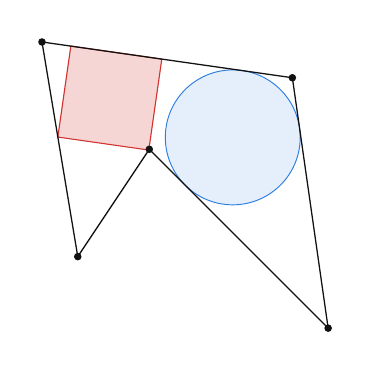
\begin{tikzpicture}[x=0.00800cm,y=0.00800cm,line join=round]
\begin{scope}\clip (250.0,-10.0) rectangle (750.0,-510.0);\path[line width=0.0120cm, draw=discC, fill=discC, fill opacity=0.12] (575.76,-184.24) circle (107.14);\end{scope}
\begin{scope}\clip (250.0,-10.0) rectangle (750.0,-510.0);\path[line width=0.0140cm, draw=squareC, fill=squareC, fill opacity=0.2] (442.38,-204.39) -- (463.02,-59.91) -- (318.54,-39.27) -- (297.90,-183.75) -- cycle;\end{scope}
\begin{scope}\clip (250.0,-10.0) rectangle (750.0,-510.0);\path[line width=0.0160cm, draw=curveC] (329.55,-373.64) -- (443.18,-203.18) -- (727.27,-487.27) -- (670.45,-89.55) -- (272.73,-32.73) -- cycle;\end{scope}
\begin{scope}\clip (250.0,-10.0) rectangle (750.0,-510.0);\path[fill=dotC, fill opacity=1] (329.55,-373.64) circle (6.00);\end{scope}
\begin{scope}\clip (250.0,-10.0) rectangle (750.0,-510.0);\path[fill=dotC, fill opacity=1] (443.18,-203.18) circle (6.00);\end{scope}
\begin{scope}\clip (250.0,-10.0) rectangle (750.0,-510.0);\path[fill=dotC, fill opacity=1] (727.27,-487.27) circle (6.00);\end{scope}
\begin{scope}\clip (250.0,-10.0) rectangle (750.0,-510.0);\path[fill=dotC, fill opacity=1] (670.45,-89.55) circle (6.00);\end{scope}
\begin{scope}\clip (250.0,-10.0) rectangle (750.0,-510.0);\path[fill=dotC, fill opacity=1] (272.73,-32.73) circle (6.00);\end{scope}
\end{tikzpicture}

\caption{The pentagon of Proposition~\ref{prop:pentagon} with its inscribed square.}
\end{figure}

It is a near-square with one deep dent. The dent matters: among quadrilaterals
obtained by moving one corner of a square to a lattice point we found none below
$\sqrt2$, in line with the $\sqrt2$ bound for convex curves (C.~Boilley, 2026; see
\cite[v255]{schulz}).

\begin{thebibliography}{9}\small
\bibitem{matschke-survey} B.~Matschke, A survey on the square peg problem,
\emph{Notices Amer.\ Math.\ Soc.} \textbf{61} (2014), 346--352.
\bibitem{matschke} B.~Matschke, On the square peg problem and its relatives,
\href{https://arxiv.org/abs/1001.0186}{arXiv:1001.0186} (2009, revised 2022).
\bibitem{pochuev} G.~Pochuev, \emph{A 10-vertex counterexample to David Bernier's sharp polygonal big peg conjecture} (2026),
\url{https://github.com/Grisha-Pochuev/sharp-big-peg-counterexample}.
\bibitem{schulz} B.~J.~Schulz, \emph{Toeplitz square-peg research}, software repository (2026),
\url{https://github.com/HiroSakuraba/Toeplitz.-Round-peg}.
\bibitem{schwartz} R.~E.~Schwartz, Rectangles, curves, and Klein bottles,
\emph{Bull.\ Amer.\ Math.\ Soc.} \textbf{59} (2022), 1--17.
\end{thebibliography}
\end{document}
